\documentclass{article}
\usepackage[utf8]{inputenc}
\usepackage[T1]{fontenc}

\title{Appunti di Introduzione all'Intelligenza Artificiale Unipi - 3 Parte}
\author{Raffaele Apetino}
\date{Marzo 2020}

\usepackage{natbib}
\usepackage{graphicx}
\usepackage[margin=3cm]{geometry}
\usepackage{amssymb}
\usepackage{xcolor}
\usepackage{proof}
\usepackage{float}
\usepackage{tipa}

\begin{document}

\maketitle

\tableofcontents{}
\clearpage

\section{Introduzione - Machine Learning}
Il problema dell'apprendimento è uno dei problemi principali dell'intelligenza sia artificiale che biologica. L'apprendimento è un obiettivo complesso con un campo di ricerca in continua crescita. L'apprendimento automatico (Machine Learning) è emerso come un'area di ricerca che combina gli obiettivi della creazione di computer in grado di apprendere. Perchè le macchine dovrebbero imparare da sole? Poichè c'è una crescente necessità di analizzare dati empirici difficili da gestire con la normale programmazione. Il ML è una via strategica per dotare intelligenza alle macchine. Il compito dell'apprendimento automatico è la creazione di sistemi intelligenti adattivi.

\subsection{Un esempio concreto}
Esempi concreti di applicazione di ML possono essere la classificazione delle email spam oppure il riconoscimento dei caratteri, dei visi o del parlato. Non ci sono regole o conoscenza pregressa per trovare la soluzione, ma diventa più facile avendo una fonte di esperienza per apprendere. Ad esempio nel riconoscimento facciale si combinano reti neurali e altri approcci di ML partendo da milioni di immagini facciali appartenenti a diversi individui. 

\subsection{Quando usare il machine learning?}
Il machine learning è una grande opportunità ma deve essere controllato. Usiamo l'apprendimento automatico quando:
\begin{itemize}
    \item non abbiamo conoscenza per spiegare il fenomeno oppure è difficile formalizzarlo
    \item abbiamo dati incerti, rumorosi o incompleti che ostacolano la formalizzazione di soluzioni
    \item ci troviamo in ambienti dinamici non conosciuti in anticipo
\end{itemize}
Abbiamo però anche dei requisiti per poter applicare Ml ai nostri problemi. E' necessaria una fonte di esperienza formativa ma è difficile raccogliere molti dati rappresentativi, per esempio, per una malattia rara. Dobbiamo anche considerare una tolleranza sulla precisione dei dati (se accettiamo di dare pochi dati in input, o poco significativi, dobbiamo anche tollerare una certa percentuale di errore, che però in alcuni casi non può essere accettata).

\subsection{Perchè usare il machine learning?}
E' una opportunità per conoscere nuovi paradigmi informatici con un approccio differente dalla programmazione standard, algoritmica e IA classica. Per trovare soluzioni approssimate a problemi difficili. Non è una metodologia approssimativa, è un approccio rigoroso per trovare funzioni approssimative per affrontare problemi complessi. 

\subsection{Sistema ML}
\begin{figure}[H]
    \centering
    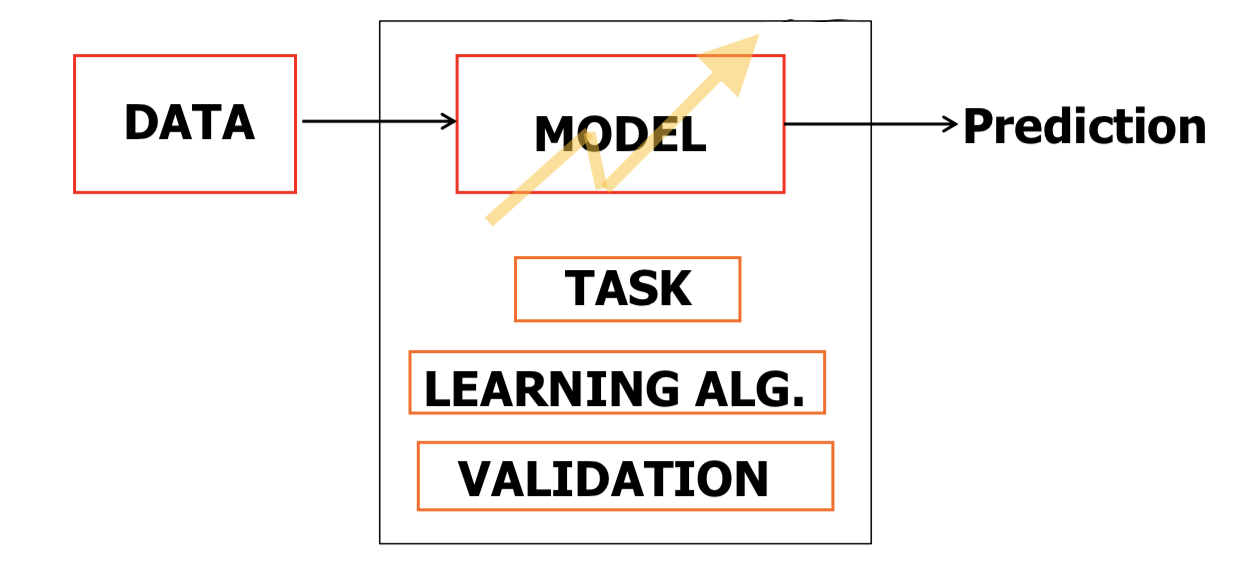
\includegraphics[scale=0.5]{Images/modelloML.png}
\end{figure}

\begin{itemize}
    \item DATA: i dati li ricaviamo dalle osservazioni del mondo
    \item MODEL: i dati passano attraverso un modello. Il modello non è fissato: ha dei parametri liberi, modificabili per fornire le predizioni in modo che siano quelle che vorremmo che fossero fornite.
    \begin{itemize}
        \item TASK: Supervised o Unsupervised Learning
        \item LEARNING ALGORITHM: algoritmo che cerca la soluzione in uno spazio di stati
        \ITEM VALIDATION
    \end{itemize}
    \item PREDICTION: è l'output restituito dal modello
\end{itemize} 
Apprendere viene visto come una approssimazione di una funzione sconosciuta ricavata dagli esempi. 

\subsubsection{Riconoscimento caratteri}
Un esempio "pilota" che possiamo fare è il riconoscimento di caratteri scritti a mano. Il problema è racchiuso nel riconoscere una funzione che passa per un insieme di punti. Come input abbiamo una collezione di immagini di caratteri scritti a mano. Il problema è costruire un modello che riceve in input queste matrici di 8x8 pixel e come output restituire la cifra riconosciuta. \newline
\begin{figure}[H]
    \centering
    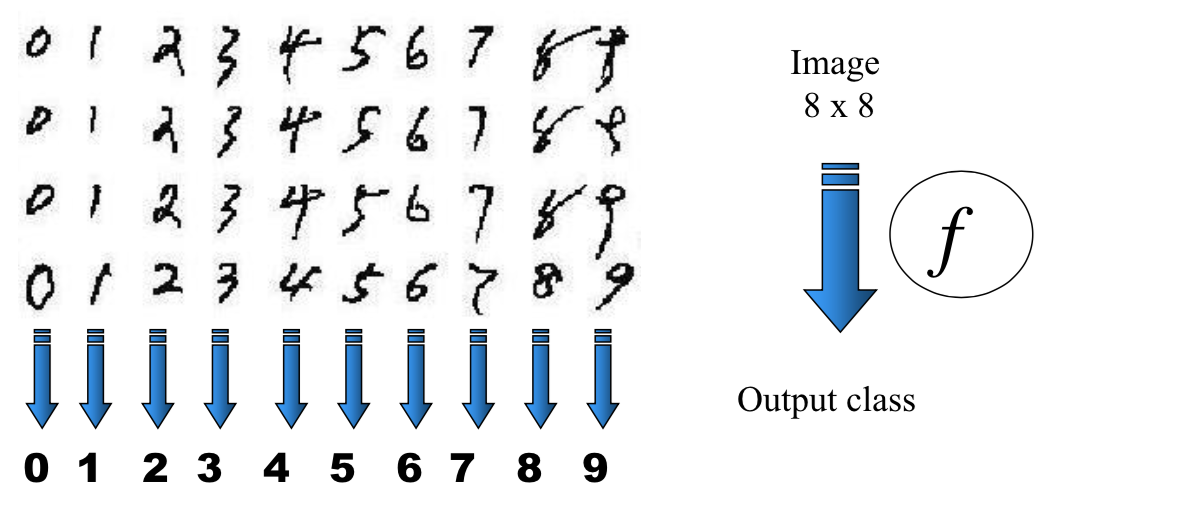
\includegraphics[scale=0.5]{Images/caratteririconoscimento.png}
\end{figure}
Non sappiamo quale sia la funzione, perché in quel caso la scriveremmo direttamente in un algoritmo. Cerchiamo quindi di approssimarla restituendo come output una classificazione della matrice. Il problema di classificazione è dato dalla formalizzazione della soluzione esatta, poiché ci possiamo trovare con dati rumorosi o ambigui. Risulta però facile raccogliere collezioni di esempi etichettati, cioè esempi con soluzioni associate. \newline
Generalizzando il problema troviamo la tecnica del Supervised Learning. In particolare abbiamo in input uno spazio x, dobbiamo costruire una funzione generale a partire dagli esempi e come output dare una categoria o valori reali. 

\subsection{TASK: Supervised Learning}
L'apprendimento supervisionato è una tecnica di apprendimento automatico che mira a istruire un sistema informatico in modo da consentirgli di elaborare automaticamente previsioni sui valori di uscita di un sistema rispetto ad un input sulla base di una serie di esempi ideali, costituiti da coppie di input e di output, che gli vengono inizialmente forniti. \newline
Vengono dati esempi di training nella forma di coppie $<input,output>$ = $<x,d>$ (esempi etichettati) per una funzione sconosciuta f. Definiamo il valore target come il valore che vogliamo ottenere come output. \newline
Bisogna trovare una buona approssimazione di f cioè una ipotesi h che può essere usata per predire l'output sui dati sconosciuti x'). \newline
L'obiettivo è una etichetta numerica o classificazione del dato. 
\begin{itemize}
    \item Classificazione: la funzione a valori discreti f(x) restituisce la presunta classe corretta per x.
    \item Regressione: consiste nell'approssimare a valori reali la funzione target.
\end{itemize}
Entrambi sono compiti di approssimazione di funzione.

\subsection{TASK: UNsupervised Learning}
L'apprendimento non supervisionato è una tecnica di apprendimento automatico che consiste nel fornire al sistema informatico una serie di input (esperienza del sistema) che egli riclassificherà ed organizzerà sulla base di caratteristiche comuni per cercare di effettuare ragionamenti e previsioni sugli input successivi. Abbiamo quindi un TR set che è un insieme di dati non etichettati, il compito è quello di raggruppare i dati in insiemi consistenti. I principali algoritmi sono:
\begin{itemize}
    \item Clustering: raggruppamento di elementi omogenei in un insieme di dati (cluster) identificando un centroide.
    \item Dimensionality reduction / Visualization / Preprocessing
    \item Modeling the data density
\end{itemize}

\subsection{MODEL}
Il compito è quello di catturare e descrivere le relazioni tra i dati. Il modello definisce la classe delle funzioni che la macchina può implementare (definisce lo spazio delle ipotesi). \newline
Concetti utili: 
\begin{itemize}
    \item Training examples: è un esempio nella forma (x,f(x)) dove x è un vettore di caratteristiche e f(x) è il valore obiettivo.
    \item Target function: la funzione obiettivo f corretta
    \item Hypotesis: è una funzione h che è ritenuta di essere simile a f. La funzione h è data in un linguaggio capace di esprimere le relazioni tra i dati.
    \item Hypoteses space: è lo spazio di tutte le ipotesi che possono essere output dell'algoritmo, è dove cerchiamo la funzione h. 
\end{itemize}
I linguaggi per h sono dei linguaggi per esprimere modelli di ML (le ipotesi h): come ad esempio la logica del primo ordine, equazioni numeriche e probabilità. \newline
\subsubsection{Esempi di Modelli}
\begin{itemize}
    \item Modelli Lineari: la rappresentazione di H definisce uno spazio continuo parametrizzato di potenziali ipotesi. Come parametro abbiamo w che è un assegnamento di ipotesi differenti: $h_w(x)=w_1x+w_0$
    \item Regole simboliche: lo spazio delle ipotesi è basato su rappresentazioni discrete, sono possibili differenti regole come ad esempio: if ($x_1$=0 and $x_2$=1) then h(x)=1 else h(x)=0
    \item Modelli probabilistici: stimare p(x,y)
    \item Approcci basati sull'istanza: prevedere il valore medio di y degli elementi più vicini (modello basato sulla memoria)
\end{itemize}

\subsection{LEARNING ALGORITHM}
Gli algoritmi di apprendimento si basano sui dati, sull'attività e sul modello. L'euristica è la ricerca delle migliori ipotesi nello spazio delle ipotesi H, cioè la miglior approssimazione della funzione obiettivo sconosciuta (ad esempio i parametri liberi del modello vengono adattati al compito da svolgere: il miglior w nel modello lineare, la miglior regola per regole simboliche, ecc...). H può non coincidere con l'insieme di tutte le possibili funzioni e la ricerca può non risultare esaustiva, per questo bisogna fare assunzioni (vedremo in seguito il ruolo dell'Inductive bias).
\begin{figure}[H]
    \centering
    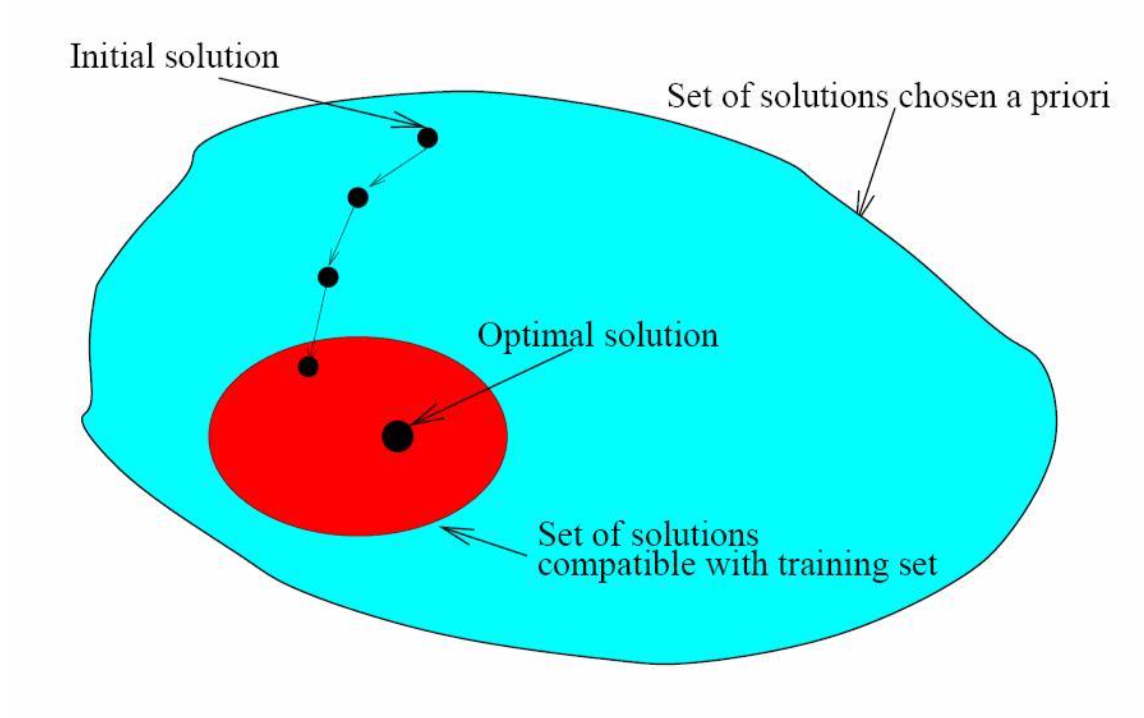
\includegraphics[scale=0.5]{Images/learningalgo.png}
\end{figure}

\subsection{VALIDATION - Generalizzazione}
L'apprendimento può essere quindi definito come la ricerca una buona funzione in uno spazio di funzioni restituito da dati conosciuti. "Buona funzione" considerando l'errore di generalizzazione (o capacità di generalizzazione) cioè quanto accuratamente il modello prevede nuovi campioni di dati. La generalizzazione è cruciale in ML $\rightarrow$ strumenti corretti di ML.
\begin{itemize}
    \item Fase di learning (training, fitting): costruire il modello dai dati conosciuti - training data and bias
    \item Fase predittiva (test): si applica a un nuovo esempio. Si prende in input x, si computa la risposta dal modello e confrontiamo l'output con il nostro target (che il modello non ha mai visto). Qui si esegue una valutazione dell'ipotesi predittiva, ad esempio la valutazione della capacità di generalizzazione (valutazione statistica del modello (quanto riesce ad essere accurato sui dati futuri). E' in questa fase che mi interessa che il modello sia accurato, non nella fase di test. Dall'altra parte la performance in ML è l'accuratezza delle predizioni stimate dal calcolo dell'errore sul test set. E' fondamentale capire che la funzione, pur sconosciuta, deve esistere. I dati di input devono avere una qualche correlazione.
\end{itemize}

%\bibliographystyle{plain}
%\bibliography{references}
\end{document}
